\documentclass[11pt]{article}
\usepackage[utf8]{inputenc}
\usepackage[T1]{fontenc}
\usepackage[spanish,es-nolayout, es-nodecimaldot]{babel}
\usepackage{enumitem}
\usepackage{array}
\usepackage{amsmath,amssymb,amsthm}
\usepackage[a4paper, left=2cm, top=2.5cm, bottom=2.5cm, right=2cm]{geometry}
\usepackage{bropd}
\usepackage{nicefrac}
\usepackage{stmaryrd}
\usepackage[nogin]{Sweave}


\newcommand{\N}{\mathbb{N}}
\newcommand{\R}{\mathbb{R}}
\newcommand{\llb}{\llbracket}
\newcommand{\rrb}{\rrbracket}

\DeclareMathOperator{\Cov}{Cov}
\DeclareMathOperator{\Var}{Var}
\DeclareMathOperator{\E}{E}

\allowdisplaybreaks
\setlength\parindent{0pt}
\renewcommand{\baselinestretch}{1.5}

\title{{\large Simulación} \\Simulación de \(\pi\) mediante variables aleatorias uniformes}
\author{Andr\'{e}s Miniguano Trujillo}
\date{\today}


\begin{document}
\input{HW16_Estimadores_pi-concordance}
\maketitle


Mediante la ley de los grandes números se puede estimar el valor de \(\pi\) por medio de un algoritmo semejante a la regla de Laplace:
    \begin{enumerate}
        \item \texttt{Fijar un número natural \(n\) suficientemente grande e inicializar \(N=0\).}
        \item \texttt{Generar \(U_i \sim \mathcal{U}(0,1)\), vectores de dos componentes para cada \(i\in \llb 1,n \rrb \).}
        \item \texttt{Si \( U_{i,1}^2 + U_{i,2}^2 \leq 1 \), entonces \(N \leftarrow N+1\) .}
        \item \texttt{Calcular \( \tilde{\pi}_1 = 4\nicefrac{N}{n} \). Este valor es una aproximación de \(\pi\).}
    \end{enumerate}

La idea es bastante sencilla: En el cuadrado de lado \(1\) y centrado en \( (\nicefrac 1 2, \nicefrac 1 2) \) generamos dos variables aleatorias uniformes (coordenadas de puntos). Luego contamos los puntos que caen dentro del círculo de radio \(1\) y centrado en \((0,0)\). Finalmente, una aproximación de \(\pi\) está dada por \(4\) veces la razón entre los puntos dentro del círculo y el número total de puntos simulados.

Pondré a prueba esta forma de simular \(\pi\):
\begin{Schunk}
\begin{Sinput}
> n <- 5000; 
> U <- runif(2*n, 0, 1);
> V <- (U[1:n]^2 + U[(n+1):(2*n)]^2)
> a <- V <= 1
> pi1 <- 4*sum(a)/n
\end{Sinput}
\end{Schunk}
Obtengo la siguiente aproximación con su respectivo error:
\[
    \begin{array}{c|c|c}
        \pi_1 & \text{error} & \text{error relativo}
        \\ \hline
        3.1608 & 0.01921 & 0.00611
    \end{array}
\]
Ahora realizaré esta prueba varias veces:
\begin{Schunk}
\begin{Sinput}
> m <- 2000;      pi1 <- rep(0,m);
> for(k in 1:m){
+     U <- runif(2*n, 0, 1);
+     V <- (U[1:n]^2 + U[(n+1):(2*n)]^2)
+     a <- V <= 1;    pi1[k] <- 4*sum(a)/n
+ }
\end{Sinput}
\end{Schunk}
Presento a continuación el histograma de frecuencia relativa de los errores relativos:
\begin{Schunk}
\begin{Sinput}
> hist(abs(pi1-pi)/pi, density=100, border="beige", main="Histograma de error relativo", 
+      xlab="", ylab="Frecuencia relativa", freq=FALSE)
\end{Sinput}
\end{Schunk}
\begin{center}
\begin{figure}[!h]
    \centering
    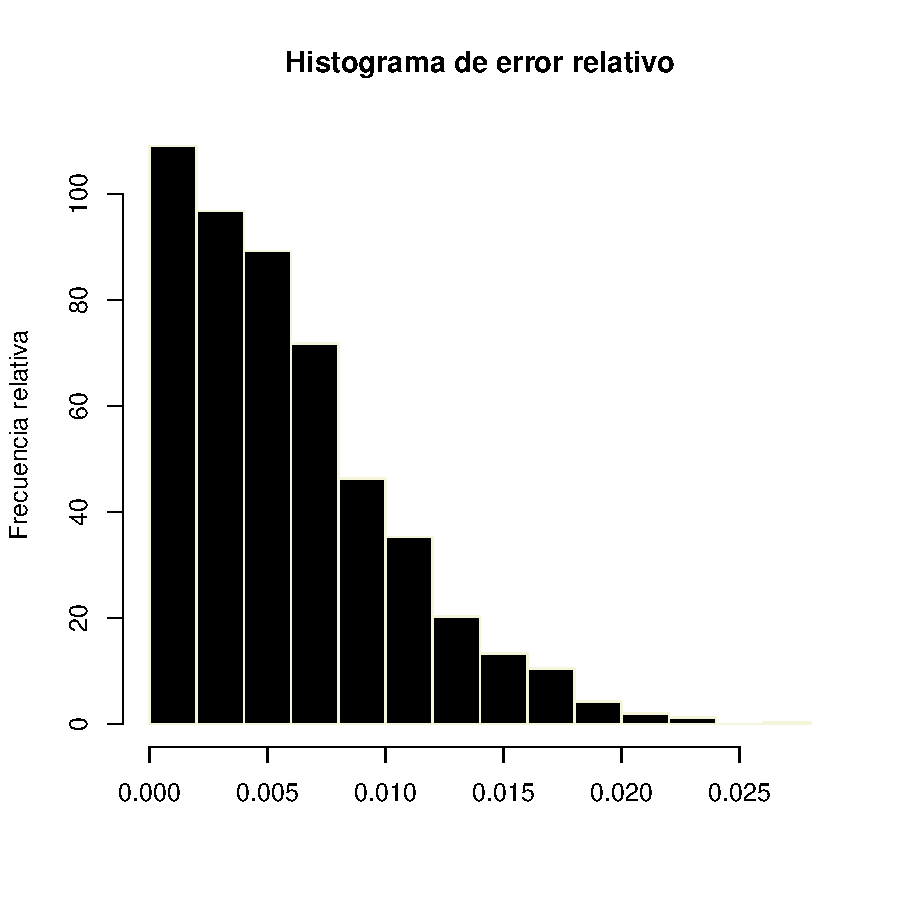
\includegraphics[width=3.25in]{EPFL-histograma}
\end{figure}
\end{center}



\end{document}
